\documentclass[12pt, a4paper, titlepage]{article}
\usepackage{amsthm}
\usepackage{amsmath}
\usepackage{amsfonts}
\usepackage{amssymb}
\setlength{\textwidth}{6.25in}
\usepackage{graphicx}
\usepackage{xcolor}
\usepackage{listings}
\lstset{numbers=none,
numberstyle=\tiny,
keywordstyle=\color{blue!70}, 
commentstyle=\color{red!50!green!50!blue!50},
frame=shadowbox,
rulesepcolor=\color{red!20!green!20!blue!20},
basicstyle=\ttfamily\small,
escapeinside=`', %将中文放在`和'之间,可以在lstlisting环境中准确的显示中文
}
\title{Financial Data Analysis Group Project\\
}
\author{Yufei Li  \\
	32014150004  \\
	\and 
	Yinan Wu \\
	32014150003 \\
	\and
	Ke Zhang\\
	32014150002\\
	\and
	Tianyunzi Chen\\
	32014020199
	}

\date{} 

\begin{document}
\maketitle

\begin{abstract}

\end{abstract}

\tableofcontents 

\section{Introduction}


\section{Data Source and Data Description}
\subsection{Data Source}

\subsection{Data Description}
We first use monthly USD/CNY exchange rate data from 1981-01-01 to 2017-06-01 to plot a trend figure shown as figure \ref{monthly}. According with the news, China used to set fixed exchange rate mechanism before 2015-07-21, the volatility of exchange rate was small. After that date, China started exchange rate regime reforming: announced a move away from the US dollar peg and used a floating exchange rate. Thus in this paper we will mainly focus on analysing exchange rate after the reform.\\ 
\begin{figure}
\begin{center}
\caption{CNY/ USD Exchange Rate using monthly data}\label{monthly}
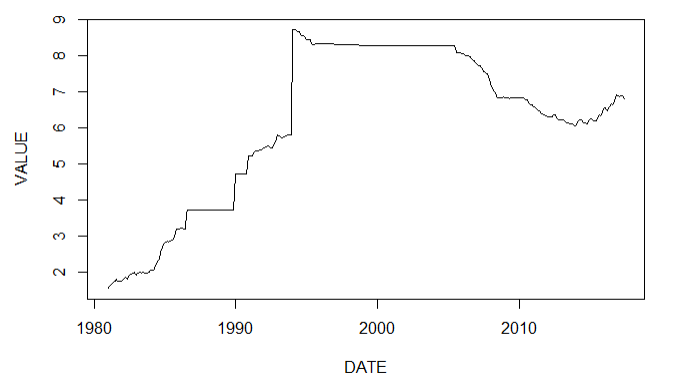
\includegraphics[width=0.6\textwidth]{monthly.png} 
\end{center}
\end{figure}

We collected the daily USD/CNY exchange rate as our data set. The data we found are already wipe out the seasonal effect so we use them directly in examining the model and further doing forecast. We divided the data into two parts one until July 21st,2016 for examine the model and the data after that date until June 9th,2017 for checking the evaluation of the models. The trend figure is shown in figure \ref{daily}.\\
\begin{figure}
\begin{center}
\caption{CNY/ USD Exchange Rate using monthly data}\label{daily}
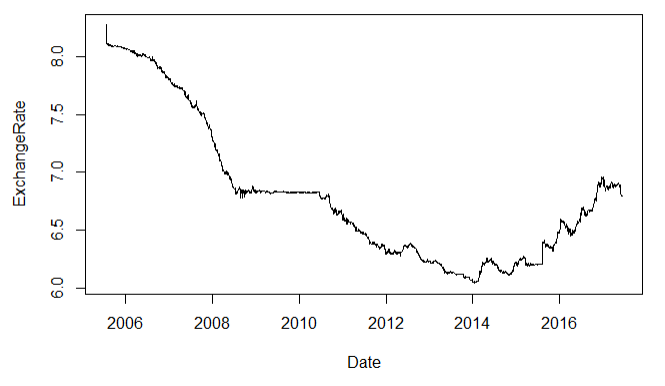
\includegraphics[width=0.6\textwidth]{daily.png} 
\end{center}
\end{figure}

\section{Model Specification}
There are usually two ways in analysing the exchange rate in time series: ARIMA model and GARCH model since they are the more general form of an ARMA model and an ARCH model. 

\subsection{ARIMA}
An ARIMA model is ARMA .\\

We first do an ADF test to check whether there exists an unit root in the serial.
\begin{lstlisting}[language=R] 
# ADF Test
origin=da$ExchangeRate
ex=origin[1:2766] # 2005-07-21 To 2016-07-21
dex=diff(ex)
m1=ar(dex,method = 'mle')
m1$order
adfTest(ex,lags=12,type=c("c"))

# Take difference
acf(dex)
pacf(dex)
\end{lstlisting}

\subsection{GARCH}

\section{Estimation and Result Analysis}

\section{Conclusions}\label{conclusions}
There is no longer \LaTeX{} example which was written by \cite{doe}.

\section{Reference}
\begin{thebibliography}{9}
\bibitem[Doe]{doe} \emph{First and last \LaTeX{} example.},
John Doe 50 B.C. 
\end{thebibliography}

\section{Appendix}
\subsection{Additional R code}
\begin{lstlisting}[language=R] 
library(readxl)
library(timeDate)
library(timeSeries)
library(TSA)
library(fUnitRoots)
library(forecast)

data <- read_excel("D:/Junior/GitHub/FDA_project_LYF/Data/MonthlyData.xls")

head(data)
dim(data)

plot(data,type="l")
\end{lstlisting}
\end{document}